\section{Projekt interfejsu użytkownika}
\subsection{Logowanie}
\begin{figure}[h!]
	\centering
	
\includegraphics[scale=0.4]{img/screens/logowanie.png}
	\caption{Ekran logowania}
\end{figure}

\subsection{Wyszukiwanie zasobu}
\begin{figure}[h!]
	\centering
	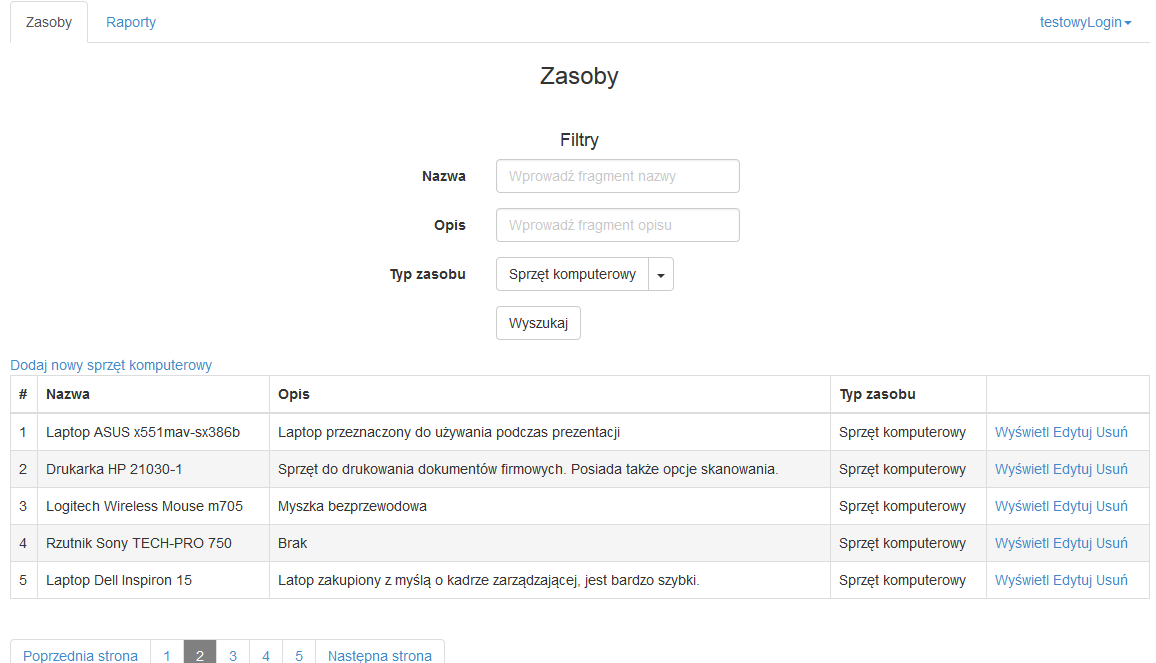
\includegraphics[scale=0.4]{img/screens/wyszZasob.png}
	\caption{Ekran wyszukiwania zasobów}
\end{figure}

\subsection{Dodawanie sprzętu komputerowego}
\begin{figure}[h!]
	\centering
	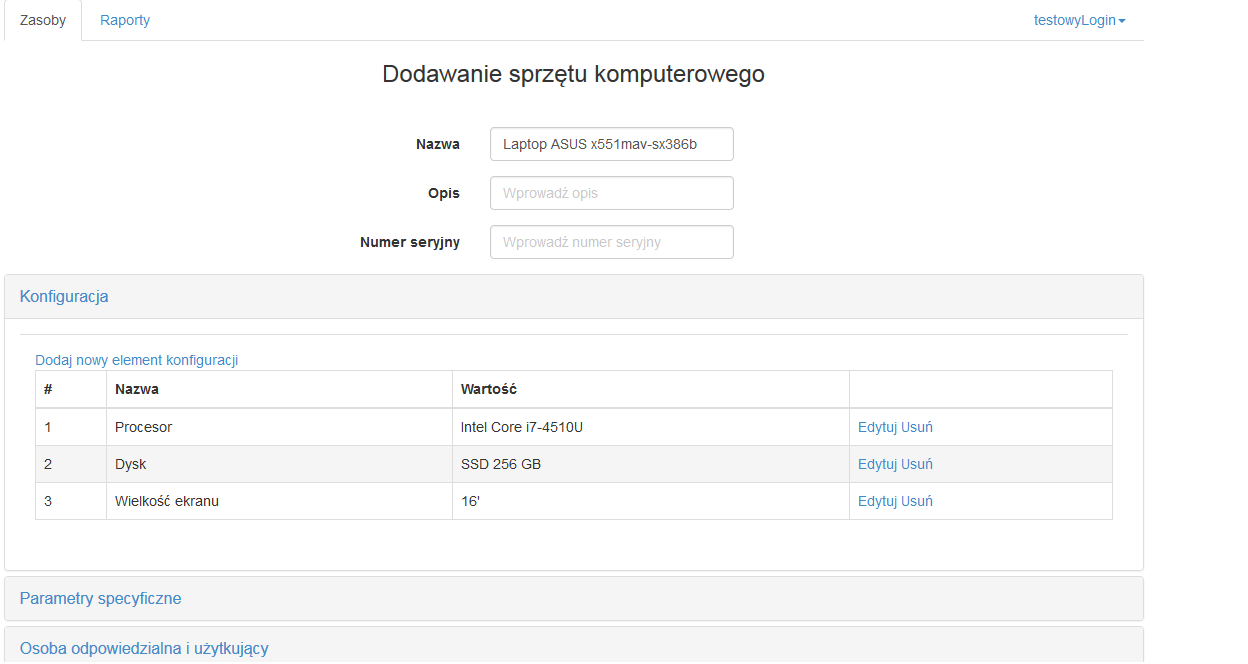
\includegraphics[scale=0.4]{img/screens/dodawanieSprzetuKomputerowego.png}
	\caption{Ekran dodawania sprzętu komputerowego}
\end{figure}

\subsection{Zapisanie informacji o użytkowniku oprogramowania}
\begin{figure}[h!]
	\centering
	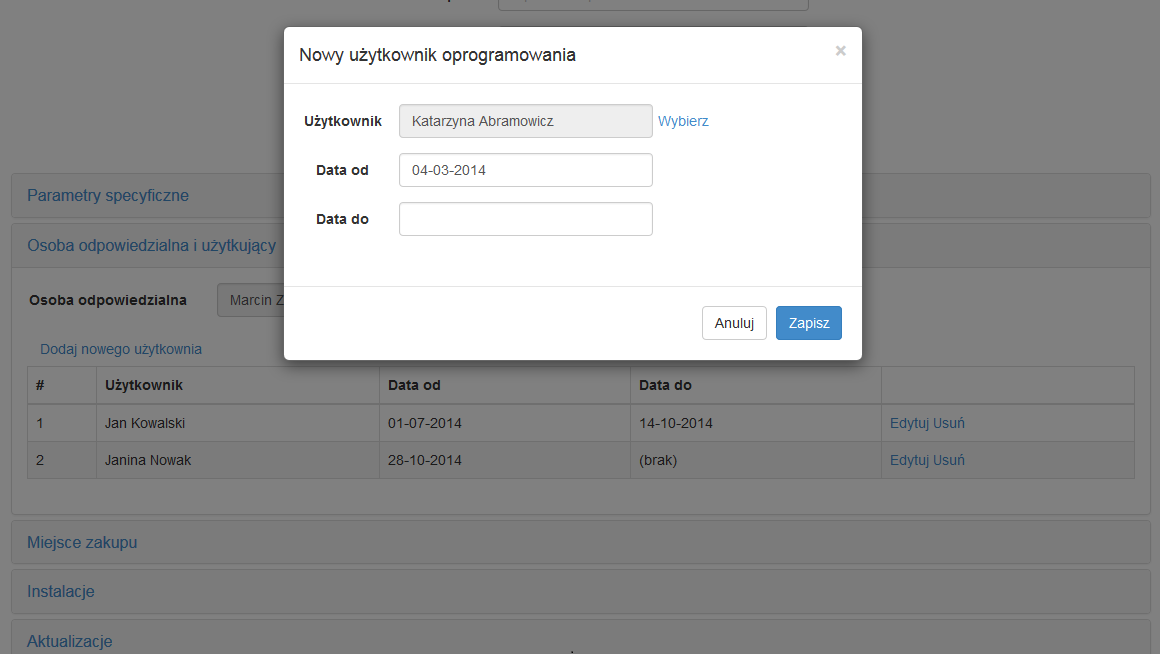
\includegraphics[scale=0.4]{img/screens/nowyUzytkownikOprogramowania.png}
	\caption{Dodawanie użytkownika oprogramowania}
\end{figure}

\subsection{Rejestracja miejsca zakupu literatury lub zasobu literaturowego}
\begin{figure}[h!]
	\centering
	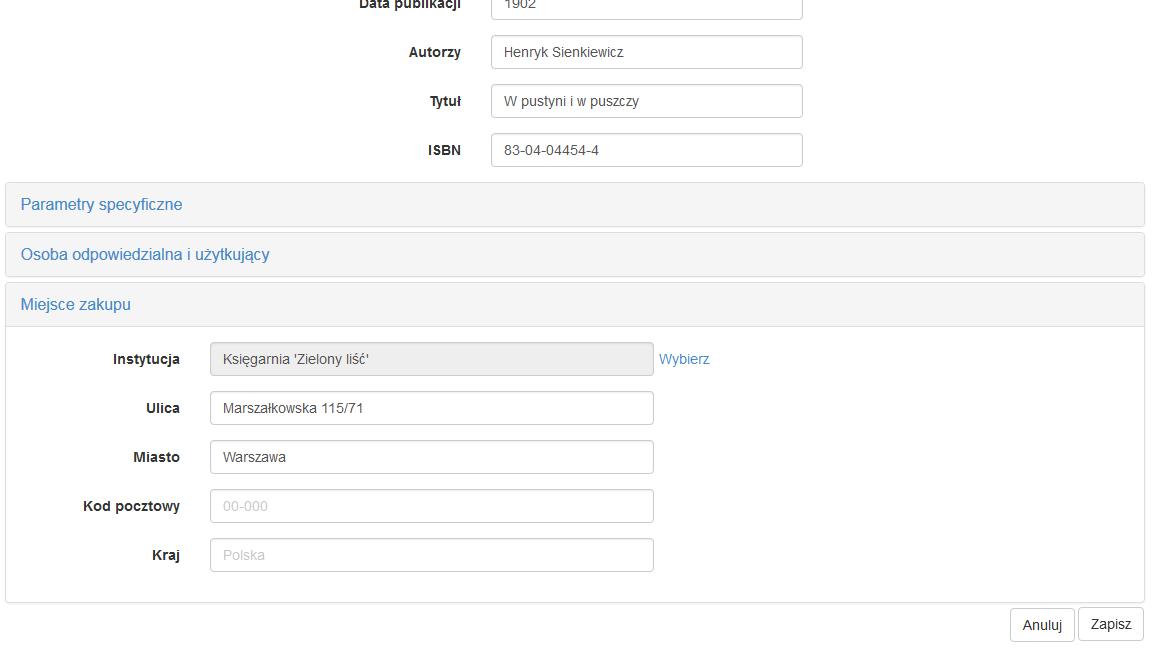
\includegraphics[scale=0.4]{img/screens/miejsceZakupuLiteratura.png}
	\caption{Edycja informacji na temat miejsca zakupu}
\end{figure}

\subsection{Edytowanie historii napraw sprzędu}
\begin{figure}[h!]
	\centering
	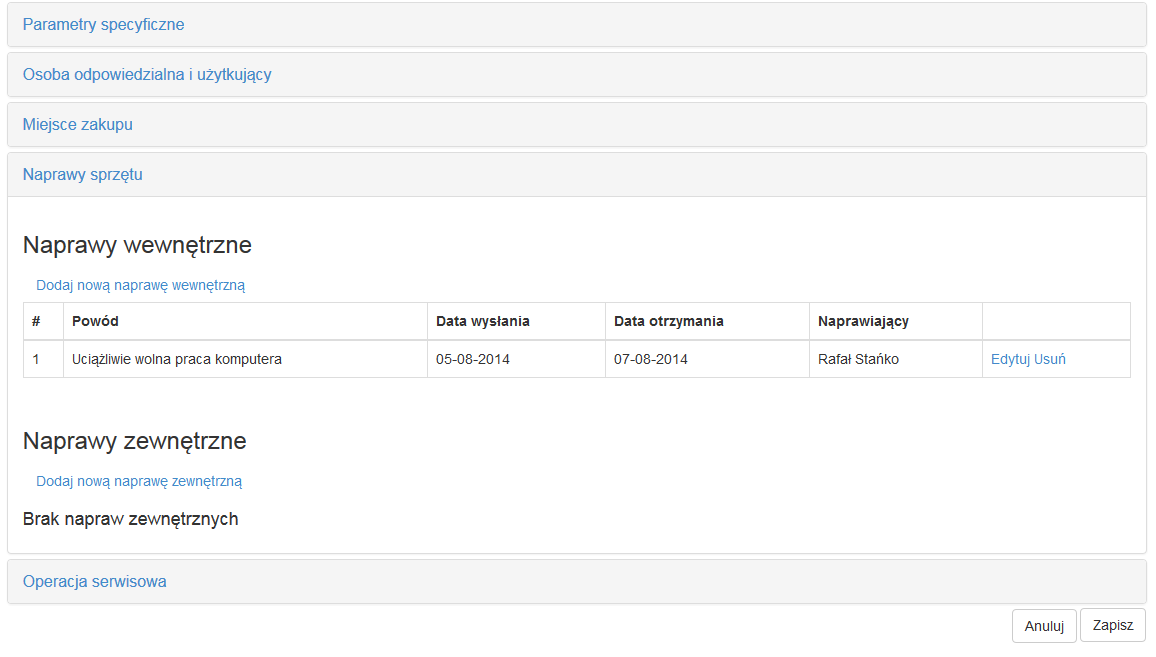
\includegraphics[scale=0.4]{img/screens/naprawyWew.png}
	\caption{Modyfikacja historii napraw sprzętu}
\end{figure}

\subsection{Prezentacja ilosci zakupionych zasobow w dzialach}
\begin{figure}[h!]
	\centering
	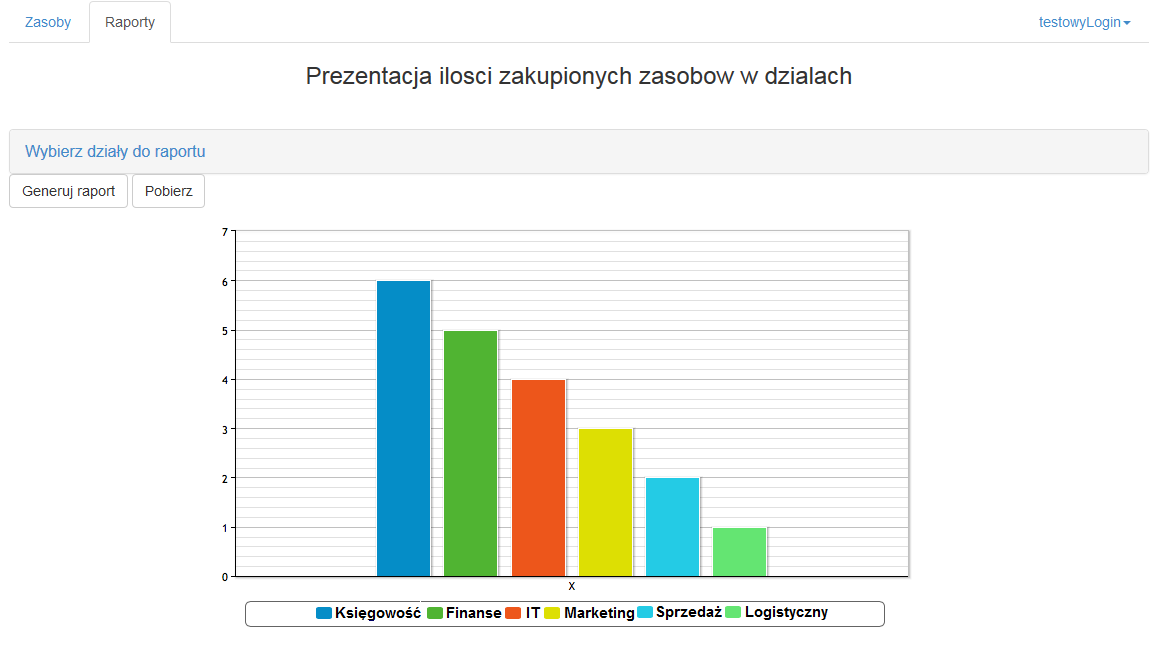
\includegraphics[scale=0.4]{img/screens/raport.png}
	\caption{Przykładowy raport - prezentacja ilosci zakupionych zasobow w dzialach}
\end{figure}
